\chapter{\textbf{DESENVOLVIMENTO}}
\label{desenvolvimento}

% Este capítulo tem por finalidade abordar todo o processo utilizado para o desenvolvimento desse projeto, relatando as principais ferramentas utilizadas e testes do algoritmo. O capítulo está dividido em seções, onde a \autoref{desenvolvimento-do-sistema} descreve o desenvolvimento do sistema, a seção \autoref{descricao-do-sistema} apresenta a descrição do sistema, etapas de funcionamento e seus riscos e restrições. A \autoref{requisitos} descreve os requisitos do sistema, a \autoref{explicacao-codigo} tem por objetivo descrever os códigos utilizados para a elaboração deste projeto e a \autoref{ambientes-de-teste} relata os ambientes de teste e os testes do software.

Este capítulo tem por finalidade abordar todo o processo utilizado para o desenvolvimento desse projeto, relatando as principais ferramentas utilizadas e testes do algoritmo. O capítulo está dividido em seções, onde a \autoref{descricao-do-sistema} apresenta a descrição do sistema, etapas de funcionamento e seus riscos e restrições. A \autoref{requisitos} descreve os requisitos do sistema, a \autoref{explicacao-codigo} tem por objetivo descrever os códigos utilizados para a elaboração deste projeto e a \autoref{testes_do_software} relata os ambientes de teste e os testes do software.

%\section{\textbf{Desenvolvimento do sistema}}
\label{desenvolvimento-do-sistema}

COMO FOI FEITO

\section{\textbf{Descrição do sistema}}
\label{descricao-do-sistema}

% Antes de descrever qualquer coisa relacionada a ferramenta, é preciso entender que o \textit{software} passa por um aprendizado de máquina para aprender os padrões de características que são necessária para atender as necessidades do projeto, que é reconhecer um jogador em campo. O \textit{haar cascade} fica responsável por realizar a classificação da imagem para obter seus padrões de características. Basicamente, o \textit{haar cascade} é alimentado manualmente por imagens aleatórias de jogadores para montar um padrão de características e em seguida, esses padrões são treinados através do \textit{machine learning}. Isso deve ser feito para que seja possível obter um modelo de busca. Pode-se definir o modelo de busca como padrão de características de jogadores de futebol americano que será utilizado para realizar a busca.

O \textit{software} apresentado no decorrer deste projeto tem por objetivo reconhecer um jogador dentro de campo utilizando as técnicas de processamento de imagem para realizar a extração de todas as características importantes que estão presentes em uma imagem.

Antes de descrever qualquer coisa relacionada à ferramenta, é preciso entender que o \textit{software} passa por um aprendizado de máquina para extrair os padrões de características que são necessária para atender as necessidades do projeto, que é reconhecer um jogador em campo. Portanto, o sistema conta com a classificação de imagem para extrair as características relacionadas aos jogadores de futebol americano, conforme representado na \autoref{fig_ext_caracteristicas}.

\begin{figure}[h]
	\caption{\label{fig_ext_caracteristicas}Etapa de extração de características de uma imagem (A) e seu padrão de características (B).}
	\begin{center}
		\resizebox{.9\linewidth}{!}{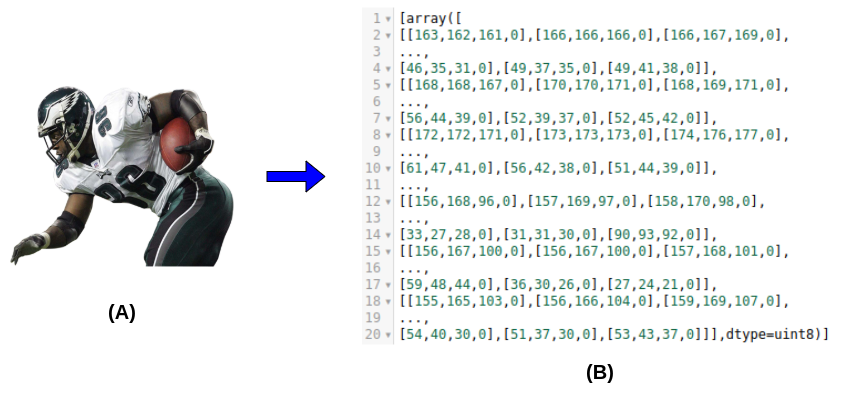
\includegraphics{6-Desenvolvimento-Projeto/imagens-desenvolvimento/conversao-de-imagem.png}}
	\end{center}
	\centering \legend{Fonte: Elaborada pelos autores.}
\end{figure}

% O \textit{haar cascade} fica responsável por realizar a classificação da imagem para obter seus padrões de características. Basicamente, o mesmo é alimentado manualmente por imagens aleatórias de jogadores de futebol americano para montar esse padrão de características. Sendo assim, pode-se definir o modelo de busca como o conjunto de padrões de características de jogadores de futebol americano que será utilizado para realizar a busca.

Quem fica responsável por realizar a classificação das imagens para obter seus padrões de características é o \textit{haar cascade}. Basicamente, o mesmo é alimentado manualmente por imagens aleatórias de jogadores de futebol americano para montar esse padrão de características. Sendo assim, pode-se definir o modelo de busca como um conjunto de padrões de características de jogadores de futebol americano que será utilizado para realizar a busca.

Em seguida, o \textit{software} passa pela etapa de \textit{machine learning} que ficará encarregada apenas de treinar o algoritmo utilizando os padrões de características. Ou seja, nessa etapa do processo, o sistema recebe como parâmetro os padrões de características extraídos na etapa anterior e analisa todos os seus pontos de interesse, montando o melhor modelo de busca.

Em seguida, o sistema recebe, através do dispositivo de captura de imagem, um vídeo em tempo real de uma partida de futebol americano.

O algoritmo realiza a análise de todos os \textit{frames}\footnote{\textit{Frames} por segundo é a taxa de atualização de imagens estáticas que formam uma cena animada dentro de um vídeo. A ilusão que nosso cérebro interpreta como movimento é feita através de vários quadros consecutivos em um curto período de tempo \cite{FRAMES2011}. \label{frames-por-segundo}} por segundo do vídeo para encontrar algo similar ao modelo de busca que foi treinado.

Caso ocorra a identificação de um jogador de futebol americano dentro do vídeo analisado, o algoritmo fica encarregado de realizar uma representação do mesmo. Essa representação será feita com um contorno verde ao redor do jogador.

\subsection{{Etapas de funcionamento do sistema}}

O funcionamento da ferramenta consiste em analisar uma imagem de um jogador objetivando adquirir todos os pontos de interesse da imagem, que servirá como parâmetro de busca para que o algoritmo seja mais eficiente quando o  mesmo for exposto a uma situação mais complexa como por exemplo, analisar um jogador com capacete.

A análise feita pelo algoritmo ocorre de forma minuciosa e utilizando técnicas de processamento de imagem. Sendo assim, após a extração de todos os pontos de interesse da imagem, o algoritmo monta um conjunto de sequências lógicas das taxas de \textit{pixels} existentes nesses pontos. Esta conversão pode ser demostrada de forma mais clara na \autoref{fig_conversao_img} da \autoref{descricao-do-sistema}.

Após a montagem do conjunto, o algoritmo utiliza um dispositivo de captura de imagem para realizar uma busca por similaridade, ou seja, o algoritmo buscará algo semelhante ao padrão montado na etapa anterior. Após a busca feita pelo \textit{software}, a detecção vai definir se existe ou não um jogador no ambiente que está sendo analisado. Se for constatado que existe um jogador e ele for igual ao modelo, a ferramenta vai apresentar o seu nome cadastrado. A \autoref{fig_fluxograma_proj} representa o fluxograma do \textit{software}.

\begin{figure}[h]
	\caption{\label{fig_fluxograma_proj}Fluxograma de funcionamento do sistema.}
	\begin{center}
		\resizebox{.9\linewidth}{!}{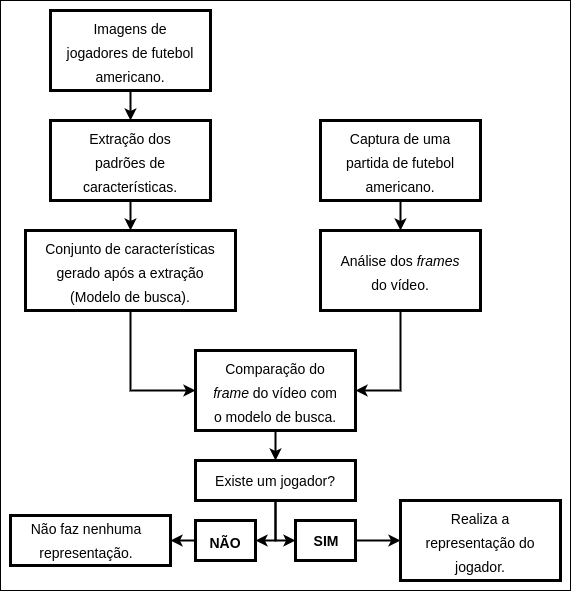
\includegraphics{6-Desenvolvimento-Projeto/imagens-desenvolvimento/fluxograma-projeto.png}}
	\end{center}
	\centering \legend{Fonte: Elaborada pelos autores.}
\end{figure}

Ao final do processo, será feito uma análise dos dados apresentados pela ferramenta. Através desses dados, pode-se obter o percentual de acertos e erros, analisando também os cenários de maior e menor eficiência.

\subsection{Restrições, riscos e exclusões do projeto}

As restrições do projeto podem ser definidas através de todos os fatores que limitam as funcionalidades do mesmo. Basicamente, são condições impostas para a elaboração do projeto que devem ser obrigatoriamente cumpridas pela equipe no decorrer do desenvolvimento do sistema. Com base nisso, as restrições deste projeto são:

\begin{itemize}
\raggedright \item Reconhecer pelo menos um jogador dentro de campo;
\raggedright \item Fazer a representação do jogador reconhecido.
% \item Somente o jogador que foi utilizado como modelo será representado. Caso algum outro jogador apareça na cena analisada, ele pode ser reconhecido como um jogador mais não terá nenhuma representação de reconhecimento, ou seja, o \textit{software} vai informar que o indivíduo é um jogador mas ele não o reconhecerá pelo nome.
\end{itemize}

Já a parte de riscos está relacionada a um evento ou situação incerta que pode afetar positivamente ou negativamente na execução do projeto. Descrevê-los é uma necessidade, para que saibamos identificar o momento certo que pode acontecer algum problema com relação ao software. Os riscos deste projeto são:

\begin{itemize}
\raggedright \item Se não houver uma boa iluminação, pode acontecer falhas no reconhecimento e até mesmo inutilizá-lo;
\raggedright \item A qualidade do sensor utilizado para capturar a imagem pode interferir no reconhecimento.
\end{itemize}

A exclusão consiste em todos os requisitos que estão explicitamente fora do projeto. Basicamente, é tudo aquilo que a equipe de desenvolvimento deixa claro que não será realizado ao longo do desenvolvimento do projeto. Sendo assim, segue a relação de requisitos que estão excluídos deste projeto:

\begin{itemize}
\raggedright \item Explicar matematicamente cada função executada;

\raggedright \item Reconhecer mais de um jogador dentro de campo;

\raggedright \item Solucionar algum possível problema identificado no processo de reconhecimento.
\end{itemize}

\section{\textbf{Requisitos}}
\label{requisitos}

\subsection{{Requisitos funcionais}}

Requisitos funcionais são responsáveis pelas funcionalidades, necessidades e características que definem um software, ou seja, eles definem o que o \textit{software} vai fazer, o seu comportamento. Os requisitos funcionais deste projeto são:

\begin{itemize}
\raggedright \item Realizar a classificação das imagens de jogadores de futebol americano.

\raggedright \item Gerar o \textit{haar cascade} com os pontos de interesses das imagens classificadas.

\raggedright \item Definir o modelo de busca a partir dos padrões de características dos jogadores de futebol americano.

\raggedright \item Realizar o treinamento do algoritmo com o modelo de busca definido.

\raggedright \item Capturar o vídeo através de um dispositivo (\textit{hardware}).

\raggedright \item Analisar cada \textit{frame} por segundo do vídeo.

\raggedright \item Identificar um jogador de futebol americano dentro de campo.

\raggedright \item Representar o jogador analisado.
\end{itemize}

\subsection{{Requisitos não-funcionais}}

Basicamente, requisitos não funcionais descrevem como o sistema fará alguma coisa. Sendo assim, os requisitos não funcionais estão relacionados ao desempenho do sistema, usabilidade, confiabilidade, restrições de projeto, manutenção e atributos da qualidade. São os seguintes:

\begin{itemize}
\raggedright \item O sistema deve ser implementado em \textit{phyton};

\raggedright \item O sistema necessita de dependências do \textit{phyton} para a sua execução;

\raggedright \item A biblioteca \textit{OpenCV} precisa estar instalada para a sua execução;

\raggedright \item O processamento da imagem será feito em \textit{hardware} próprio;

\raggedright \item O sistema requer grande processamento de \textit{hardware};

\raggedright \item Para a definição de um novo modelo, o sistema precisa passar por uma manutenção dos parâmetros de busca e, consequentemente, um novo treinamento da ferramenta;

\raggedright \item Para que o sistema possa ser executado, é necessário realizar comandos via terminal;

\raggedright \item O \textit{software} precisa de um dispositivo de captura de imagem como, por exemplo, uma \textit{Web Cam};

\raggedright \item O \textit{software} deve poder ser executado em \textit{Windows} e \textit{Linux}.

\end{itemize}

\section{\textbf{Explicando o código}}
\label{explicacao-codigo}
\definecolor{cinza}{rgb}{0.95,0.95,0.95}

Antes de explicar o código por trás do desenvolvimento deste projeto, é preciso informar que para executá-lo é necessário instalar a linguagem de programação \textit{Python} e suas dependências.

Para iniciar a codificação do algoritmo em \textit{Python}, é importante realizar a importações das bibliotecas necessárias para realizar o procedimento de reconhecimento. A biblioteca \textit{cv2} é a \textit{OpenCV}; a \textit{NumPy} fica responsável por realizar cálculos de vetores multidimensionais; a \textit{argparse} verifica e atribui os argumentos que são esperados; já a \textit{imutils} é responsável por converter a imagem em uma matriz.

\begin{minted}[linenos=true, mathescape, bgcolor=cinza]{python}

import cv2
import numpy as np
import argparse
import imutils

\end{minted}

Também é necessário importar os módulos da biblioteca \textit{imutils}.

\begin{minted}[linenos=true, mathescape, bgcolor=cinza]{python}

from __future__ import print_function
from imutils.object_detection import non_max_suppression
from imutils import paths

\end{minted}

Em seguida, o algoritmo deve ser programado para construir os argumentos necessários para iniciar o reconhecimento e analisar esses argumentos.

\begin{minted}[linenos=true, mathescape, bgcolor=cinza]{python}

ap = argparse.ArgumentParser()
ap.add_argument("-i", "--images", required=True,
    help="path to images directory")
args = vars(ap.parse_args())

\end{minted}

Agora é necessário iniciar o descritor \textit{HOG - Histogram of Oriented Gradients} (Histograma de Gradientes Orientados). Basicamente, o \textit{HOG} utiliza cálculos matemáticos extremamente complexos que serve para classificar dados da imagem e gerar um \textit{haar cascade} com suas configurações.

\begin{minted}[linenos=true, mathescape, bgcolor=cinza]{python}

hog = cv2.HOGDescriptor()
hog.setSVMDetector(cv2.HOGDescriptor_getDefaultPeopleDetector())

\end{minted}

Para o melhor desempenho do algoritmo, foi criado uma pasta local contendo todas as imagens necessárias para realizar a extração dos padrões de características dos jogadores de futebol americano. Sendo assim, o trecho de código a seguir serve para ler todas estas imagens que estão dentro da pasta \textit{images} localmente.

\begin{minted}[linenos=true, mathescape, bgcolor=cinza]{python}

imagePaths = list(paths.list_images(args["images"]))

\end{minted}

A partir desta etapa, o algoritmo vai executar uma estrutura de repetição para analisar todas as fotos alocadas na variável \textit{imagePaths} utilizada no trecho de código acima.

Sendo assim, o primeiro laço da estrutura de repetição fica responsável por carregar e redimensionar a imagem para reduzir o tempo de detecção. Em seguida, ele melhora a precisão da detecção da imagem para melhorar a extração de características.

\begin{minted}[linenos=true, mathescape, bgcolor=cinza]{python}

for imagePath in imagePaths:
	image = cv2.imread(imagePath)
	image = imutils.resize(image, width=min(400, image.shape[1]))
	orig = image.copy()

\end{minted}

Em seguida, ele tenta detectar se existe uma pessoa na imagem analisada.

\begin{minted}[linenos=true, mathescape, bgcolor=cinza]{python}

    (rects, weights) = hog.detectMultiScale(image, winStride=(4, 4),
        padding=(8, 8), scale=1.05)

\end{minted}

Apos isso, a segunda estrutura de repetição que está alocada dentro da primeira, fica responsável por delimita os locais onde contem os pontos de interesse dentro da imagem analisada, ou seja, o algoritmo seleciona as áreas de interesse que serão utilizadas como parâmetro de busca.

\begin{minted}[linenos=true, mathescape, bgcolor=cinza]{python}

    for (x, y, w, h) in rects:
	cv2.rectangle(orig, (x, y), (x + w, y + h), (0, 0, 255), 2)

\end{minted}

Em seguida, o \textit{software} realiza a técnica de supressão não máxima na imagem, ou seja, ele realiza a técnica de detecção de bordas para identificar os \textit{pixel} de maior intensidade e, em seguida, ele realiza a técnica de supressão para eliminar os \textit{pixels} que não possuem valores próximos aos da borda.

\begin{minted}[linenos=true, mathescape, bgcolor=cinza]{python}

    rects = np.array([[x, y, x + w, y + h] for (x, y, w, h) in rects])
	pick = non_max_suppression(rects, probs=None, overlapThresh=0.65)

\end{minted}

A terceira estrutura de repetição fica responsável por montar uma delimitação do indivíduo detectado na imagem analisada.

\begin{minted}[linenos=true, mathescape, bgcolor=cinza]{python}

    for (xA, yA, xB, yB) in pick:
		cv2.rectangle(image, (xA, yA), (xB, yB), (0, 255, 0), 2)

\end{minted}

Apos os procedimentos, o algoritmo fica responsável por desenhar as correspondências de informações contidas entre as imagens analisadas.

\begin{minted}[linenos=true, mathescape, bgcolor=cinza]{python}

    filename = imagePath[imagePath.rfind("/") + 1:]
	print("[INFO] {}: {} original boxes, {} after suppression".format
		(filename, len(rects), len(pick)))

\end{minted}

Por fim, o sistema mostra na tela a imagem analisada e os pontos de interesse que ele achou dentro da mesma. Na outra imagem, o \textit{software} mostra o que ele achou de semelhante após a análise.

\begin{minted}[linenos=true, mathescape, bgcolor=cinza]{python}

cv2.imshow("Before NMS", orig)
cv2.imshow("After NMS", image)
cv2.waitKey(0)

\end{minted}

A \autoref{fig_comparativo_img} descreve o que o sistema faz com a imagem e o seu resultado.

\begin{figure}[h]
	\caption{\label{fig_comparativo_img}A imagem (A) é a original, e as representações em vermelho são seus pontos de interesse. A imagem (B) é o resultado da detecção por bordas e seus pontos similares com a imagem (A).}
	\begin{center}
		\resizebox{.9\linewidth}{!}{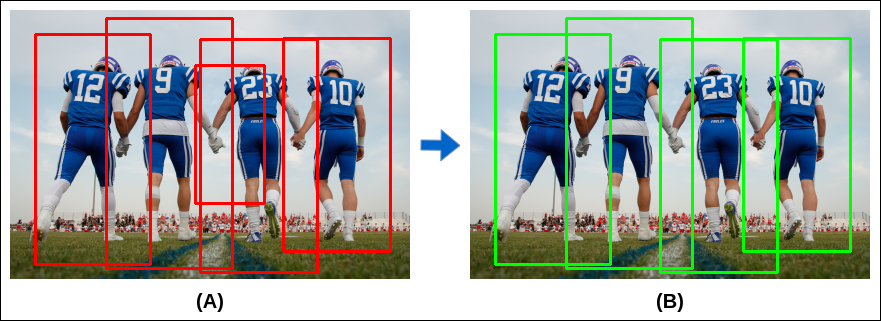
\includegraphics{6-Desenvolvimento-Projeto/imagens-desenvolvimento/comparativo_imagem.png}}
	\end{center}
	\centering \legend{Fonte: Elaborada pelos autores.}
\end{figure}

\subsection{{Testes do \textit{software}}}


\section{\textbf{Análise dos resultados}}

Para resumir os resultados obtidos nos testes de \textit{software}, foi feito uma tabela que tem por finalidade representar quais foram os ambientes de testes que o algoritmo foi submetido. Sendo assim, a \autoref{resultado_de_testes} mostra os resultados dos testes do algoritmo.

\begin{table}[h]
\centering
\caption{Resumo dos resultados dos testes}
\label{resultado_de_testes}
\begin{tabular}{l|l} 
\hline
\hline
\multicolumn{1}{l|}{Ambiente de Teste} & \multicolumn{1}{l}{Resultado}  \\ 
\hline
Partida de futebol americano & Positivo\\
Partida de futebol americano & Negativo\\
Jogador parado & Positivo\\
Jogador em movimento & Intermediário\\
Jogador de frente & Positivo\\
Jogador de costas & Positivo\\
\hline
\hline 
\end{tabular}
\end{table}